% !TEX root = ../thesis-example.tex
%
\chapter{System Setup}
\label{ch:system-setup}

The following section describes the hard- and software components used for the 
thesis and results. All demonstrations have been performed on that environment. 
All dependencies have been explicitly marked to allow a similar, but not exact, 
setup to reproduce these results.

\begin{figure}[htb]
	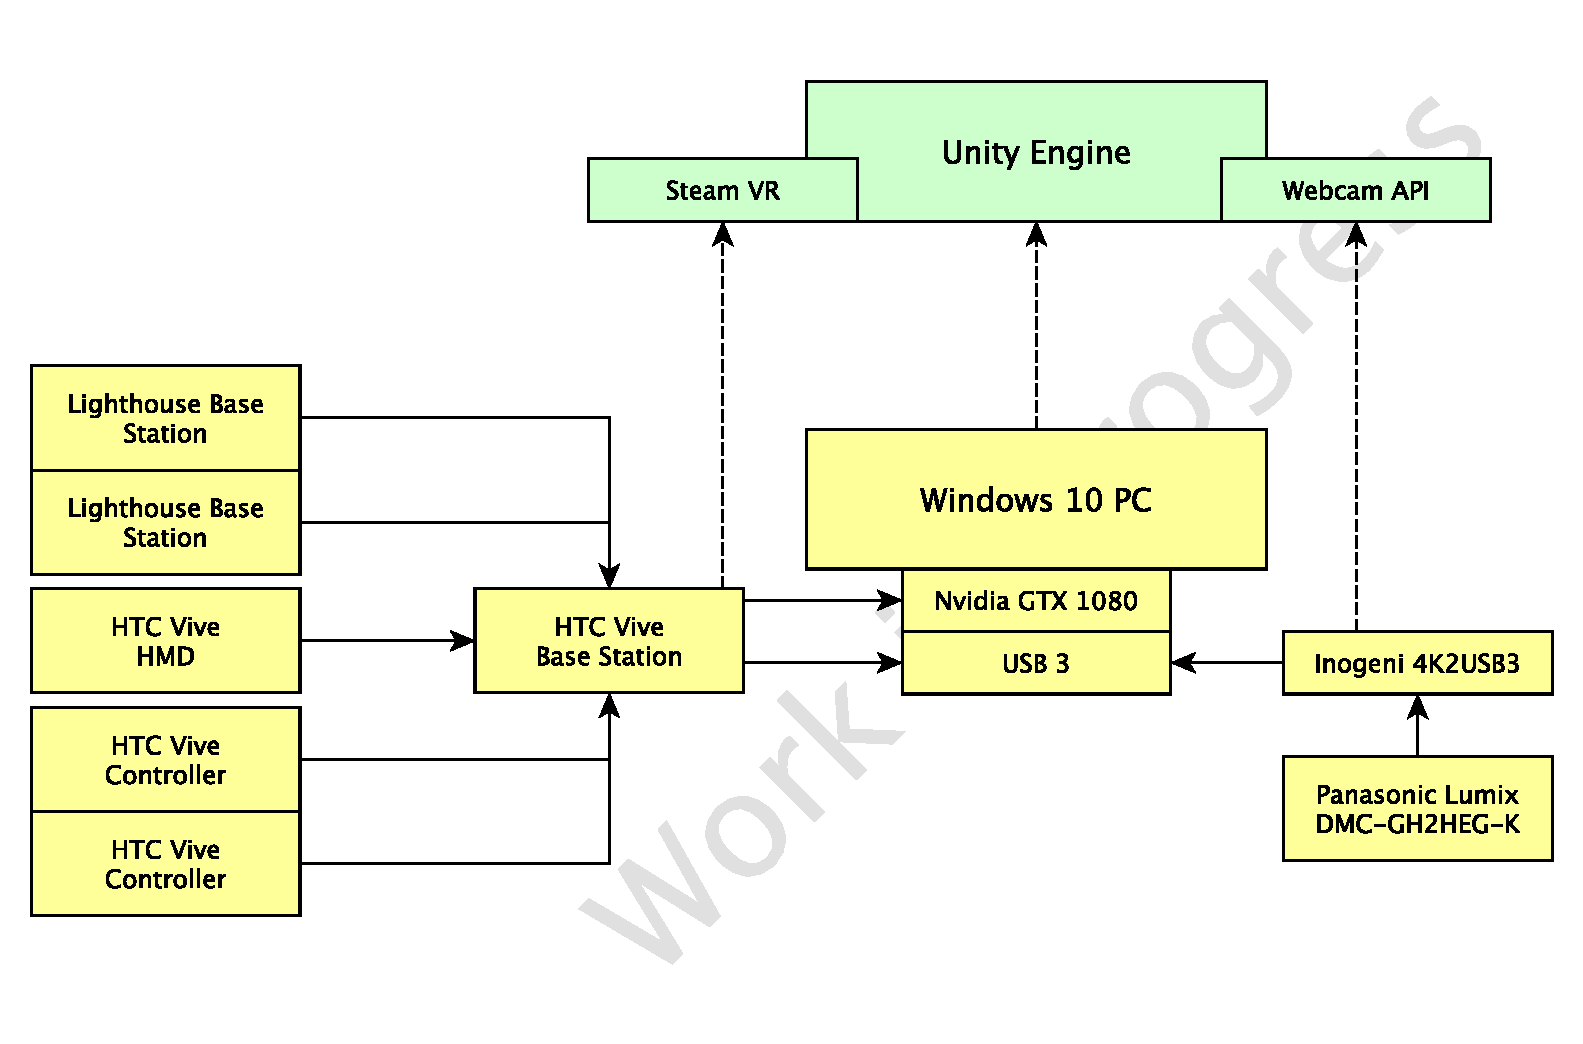
\includegraphics[width=\textwidth]{gfx/System-Components}
	\caption{Diagram of hard- and software components.}
	\label{fig:system-components}
\end{figure}

\section{Hardware Configuration}
\label{sec:hardware-config}

The hardware configuration is split in three main parts:
\begin{my_list}
	\item Windows PC Workstation
	\item Virtual Reality Tracking Solution
	\item Motion Video Input Feed
\end{my_list}

Each individual configuration is basically interchangeable with other systems, 
as long as predefined conditions are met. Each condition is listed first in 
each subsection.

\subsection{PC Workstation}

As the software is built in the Unity Engine, the workstation is limited to 
either Windows or Mac OS X systems the only requirement - besides being 
powerful enough to render the 3D scenes - is two USB3 ports to ensure enough 
data throughput for the video and virtual reality solution, as well as two 
video outputs for a monitor and its headset.
\newline
The configuration used here is:
\begin{lstlisting}
	CPU: Intel i7-4700K @ 4.00 GHz
	RAM: 16GB DDR4
	GPU: Nvidia GTX 1080
\end{lstlisting}
% TODO: Add missing specs of the system.

This system configuration is to date a high end workstation that has an 
abundance of render performance, allowing it to process and keep enough 
framebuffer for the operation described further in.
\todo[inline]{weak text.}

\subsection{Inogeni 4K2USB3}
The Ingoeni 4K2USB3 converter is a standalone box that allows to receive any 
HDMI source and converts it as external webcam video feed. It's advantage is by 
the arbitrary choice of video cameras and a very simple integration with any 
software. With the help of the converter box it's possible to request a webcam 
as video resource and process that video feed as a texture on the GPU. 

\subsection{Panasonic GH2 Systemcamera}
This camera provides a direct video feed via HDMI with low latency. It can 
directly feed into the Inogeni 4K2USB3 and produces a stable, high quality 
video feed with a low signal to noise ratio in well lit environments.
\todo[inline]{still unclear if this remains the target camera.}

\subsection{HTC Vive with Controllers and Lighthouses}
The current best virtual reality and tracking device is the HTC Vive. It 
includes two infrared sending stations called "Lighthouse", two Vive 
Controllers and a Headset, both systems with 6 degrees of freedom (6DOF) 
tracking. The tracking system is a blackbox, in which only the transformation 
matrices for the hand controllers and the HMD can be accessed. By default this 
transformation has a normalized length of 1 unit to 1 meter. Designing scenery 
and sense of size is therefore rather easy. The data providing is done by a 
library called "SteamVR for Unity", which makes the usage in engine transparent.

\subsection{Vive Controller Tripod Mount}
Most cameras have a standardized way of mounting tripods. Since the Vive 
controllers have no reference plane and minuscule differences in mounting 
angles changes the projection parameters to noticeable effects, it was 
necessary to build a mount for the camera to keep controller and video 
equipment transformation in sync, I built a mount that fits on tripod 
attachment points and keeps the controller locked in the same position.
\todo[inline]{add example for incorrect projection and model of mount}

\section{Software}

The software of choice is Unity3D, which is free for students, non-profit 
organizations and small studios. It provides a \todo[inline]{interrupted 
writing}